\chapter{Introduction}

One of the main problems in the effective visualization of graphs is the avoidance or minimization of edge crossings in graph drawings. Very active research has been done around this problem, with works in mathematics, computer science, data visualization, and psychological user studies.

Becker et.\ al.~\cite{Becker} first propose a radically new approach to avoid edge crossings in two-dimensional drawings of non-planar graphs. They were trying to visualize overload of the AT\&T long-distance telephone network when in 1989 the San Francisco Bay area was hit by an earthquake. They were interested in where network congestion occurred and which connections carried the most traffic. In the drawing of the network, long intercontinental connections covered most of the underlying map of the U.S.\ and any problems below. They solved this problem by drawing only a certain fraction of each edge.

More recently, Burch et.\ al.~\cite{Burch} compared the readability of drawings of directed graphs drawn with partial edges to conventional drawings. They conducted a controlled user experiment with 42 participants to uncover differences in accuracy and completion time for three different tasks: 
\begin{itemize}
	\item [T1)] identifying the existence of an edge, 
	\item [T2)] deciding whether a pair of vertices is connected by a path of length two,
	\item [T3)] identifying the vertex with the highest out-degree.
\end{itemize}
With decreasing the edge length, the error rates decreased for Task 3 and increased for the two other tasks. The partially drawn edges resulted in shorter task completion times for all tasks and nearly all graph sizes. There was an interesting drop in the time required to complete Tasks 1 and 2 where the edges were shortened to about 75 percent. This drop in time can indicate that about 75 percent of the length of the drawn edges provides an optimal balance between clutter reduction and edge perception under the conditions and test parameters chosen.

Bruckdorfer and Kaufmann~\cite{BK} were the first to formalize the problem of drawing graphs with partial edges and introduce the concepts of symmetry and homogeneity. In this work, we consider a symmetric and homogeneous problem. We define a {\it partial drawing}, where the edges of the graph are represented by straight lines, without drawing the central halves of the lines. Additionally, we require that there be no crossings between such drawn edges. A partial drawing is said to be {\it symmetrical} because the drawn parts of the edge are of equal length. Due to the symmetry of the partial drawing, it is easier to identify the existence of an individual edge. We also say that a partial drawing is {\it homogeneous} because the proportion of the drawn part of an edge is the same for all edges. Due to the homogeneity, starting from the first end, it is easier to find the second end of the edge, because the distance to the second end can be inferred from the lengths of the drawn parts of the connection. Also, by drawing quarters of the edge, we equalize the proportions of the drawn and deleted parts. Bruckdorfer and Kaufmann also wanted to answer the question of which graphs can be drawn as a partial drawing. They showed that any complete graph $K_{n}$ for $n = 1,2 ..., 11$ can be drawn as a partial drawing. Through experimentation or local optimization, they showed that it is also possible to draw $K_{16}$ as a partial drawing. The result is shown in Figure~\ref{fig: K_16}.

\begin{figure}
  \centering
  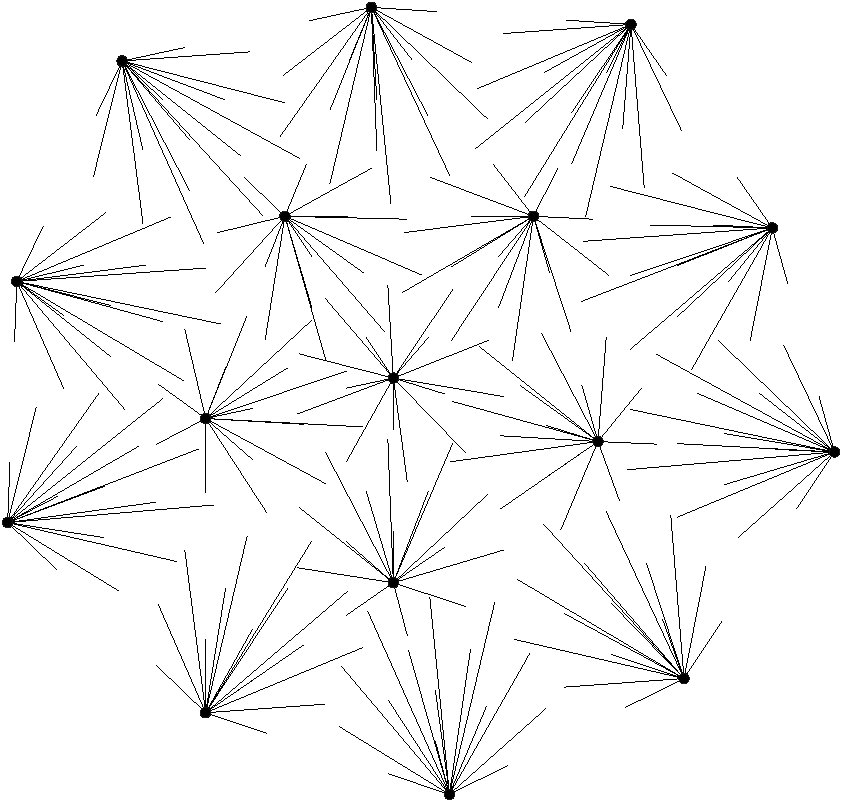
\includegraphics[width=.3\textwidth]{./figures/K16PEDCropped.pdf}
  \caption{Partial drawing of $K_{16}$}
  \label{fig: K_16}
\end{figure}


Bruckdorfer et.\ al.~\cite{Bruckdorfer} have shown that the upper bound on the number of vertices of a complete graph that can be drawn as a partial drawing is finite. They started with a simple proof that it is not possible to draw a partial drawing of a complete graph on 17 vertices in one-sided convex position. According to the result of Erd\H{o}s and Szekeres~\cite{Erdos}, any set with more than
\begin{equation*}
  \binom{2k-4}{k-2}
\end{equation*}
points, contains a subset in the one-sided convex position with $k$ points. If we insert $k = 17$ into the above expression, we arrive at the first estimate that for each
$$
  n > \binom{30}{15} = 155117520
$$
we cannot draw a partial drawing of a complete graph on $n$ vertices. They then significantly improved this estimate using the coordinate division of the plane on which the vertices of the complete graph are drawn into rectangles and showed that it is not possible to draw a partial drawing of the complete graph on 241 or more vertices.

In this work, we improve the estimate by a factor of more than two. We show that it is not possible to draw a partial drawing of the complete graph on 102 or more vertices. The main ideas are two. First, we use a different division of the plane on which the points of the graph are located. The coordinate division into rectangles has no real connection with the geometry of the partial drawing. Our approach to finding a suitable division was based on rays from pre-selected points of the drawing. In this way, the boundaries of the division are parallel to at least one of the partial edges. The resulting division has a geometry that is similar to the geometry of the partial drawing. However, the division now depends on the relative position of the pre-selected boundary points. The second idea is to analyze the entire drawing of the graph according to the location of three, sometimes even four, points of the drawing and not only two as in the previous estimates.

% TODO
In the next chapter, Preliminaries, we first define the basic concepts and establish terminology and notation. More important terms are indicated by the headings of the sections in which we define these terms. We then present the main tools (that follow from the fact that the graph $K_{3,3}$ is not planar), which allow us to control the number of points of a partial drawing. We prove the claims and theorems that serve as building blocks in the construction of the estimates.

In the third chapter, Estimates, we first define the frame in which all the points of the partial drawing lie. The frame is divided according to the three pre-selected boundary points into the following regions:
\begin{itemize}
  \item central triangle,
  \item left and right triangle and
  \item lower quadrilateral.
\end{itemize}
For each region, we derive an upper bound on the number of points in the partial drawing that lie in this region. We can assume that the central triangle is equilateral and use symmetry several times, which makes it easier to arrive at an estimate. It is different with the remaining areas. The left and right triangles are divided into cells so that each cell contains at most one point of the partial drawing. The position and number of these cells, however, vary according to the position of the selected boundary point. In addition to the cells, we use other types of polygons to divide the lower quadrilateral, which again depend on the position of the selected boundary point.

In the final chapter, Conclusion, we combine the derived bounds into the final result and present it graphically. Due to the dependence of the division on the mutual position of the boundary points, the result of the analysis is a function that represents the estimate for the upper bound on the maximum possible number of points of partial drawing. The illustrations show the division of the frame in the critical position of the boundary points, where this function reaches a maximum. We evaluate the result and suggest possible further guidelines for analysis. Appendix A provides the source code of the major calculations that helped us make the estimates.
